%
% teil1.tex -- Beispiel-File für das Paper
%
% (c) 2020 Prof Dr Andreas Müller, Hochschule Rapperswil
%
% !TEX root = ../../buch.tex
% !TEX encoding = UTF-8
%
\section{Grundlage zur Berechnung der Balkengleichung
\label{balken:section:teil1}}
\subsection{Grundbegriffe der Mathematik}
\textbf{Ableitung}
Die Ableitung einer Funktion f(x) ergibt die Steigung der Funktion f(x) an der Stelle x.
Das bedeutet, dass die Ableitung einer Funktion der Grenzwert des Differenzen-quotienten dieser Funktion f(x) ist.
Ableitungen werden mit einem «’» gekennzeichnet (z.B. f’(x)).

\textbf{Differenzialgleichung (DGL)}
Differentialgleichungen, kurz DGL, sind mathematische Gleichungen, die die Beziehung zwischen einer unbekannten Funktion und ihren Ableitungen beschreiben.
Mit anderen Worten, sie beschreiben, wie sich eine Funktion in Bezug auf eine oder mehrere unabhängige Variablen verändert.
Differentialgleichungen werden in verschiedenen Bereichen der Naturwissen-schaften, Ingenieurwissenschaften und Mathematik verwendet, da sie oft Phä-nomene beschreiben, die sich im Laufe der Zeit oder im Raum ändern.

\textbf{Euler-Lagrange-Differenzialgleichung}
Die Euler-Lagrange-Differentialgleichung ist bei der Variationsrechnung, eine bedeutende Gleichung.
Es wird verwendet, um die Extremwerte von Integralen zu finden, die eine be-stimmte Form besitzen und als Variationsprobleme bekannt sind.

\textbf{Integration}
Die Berechnung von Integralen befasst sich mit der Bestimmung von Ergebnissen über die Fläche unter beliebigen Funktionen.
Diese Flächen können zwischen den Achsen und einer Funktion, zwischen zwei Funktionen oder auch die Oberfläche von Rotationskörpern umfassen, was zur Berechnung von Volumina führt.

\textbf{Lagrange-Funktion}
Ist einen Ansatz, um Optimierungsaufgaben mehrdimensionaler Funktionen mit Nebenbedingungen zu lösen.
Das ursprüngliche Funktion mit Lagrange-Multiplikatoren kombiniert, dabei erhält man die Lagrange Funktion.
Durch das Ableiten der Lagrange-Funktion und danach das Nullsetzen diese Ableitung erhält man die Lösung zu dem Problem.

\textbf{Partielle Differentialglei-chung (PDGL)}
Eine partielle Differentialgleichung (PDGL) ist eine Art von Differentialgleichung, die partielle Ableitungen von unbekannten Funktionen enthält.
Diese Gleichungen werden verwendet, um Phänomene zu erklären, die von meh-reren unabhängigen Variablen abhängen.
Im Gegensatz zu gewöhnlichen Differentialgleichungen, bei denen nur nach einer einzigen Variablen differenziert wird, wird in partiellen Differentialgleichungen eine Funktion von mehreren Variablen betrachtet und nach diesen Variablen partiell abgeleitet.

\textbf{Variationsproblem}
Variationsprobleme sind Probleme, bei denen man versucht die Extremwerte einer Funktion zu finden, die von anderen Funktionen abhängen.
Dabei ist es wichtig zu bemerken, dass diese Problemstellung unendliche dimensi-onale Minimierungsaufgaben ist.
Ein bekanntes Beispiel für Variationsprobleme ist das «Brachistochrone-Problem».

\subsection{Grundbegriffe der Baustatik}
\textbf{Balken}
Eine «Balke» ist ein langer, schmaler Körper, der hauptsächlich Querkräften sowie Biegebelastungen ausgesetzt ist.
Balken können unterschiedliche Formen annehmen.

\textbf{Balkengleichung}
Die Balkengleichung (auch als Euler-Bernoulli-Balkengleichung (EBB) bekannt) beschreibt das Biegeverhalten eines Balkens unter der Einwirkung von Querkräf-ten und / oder Momenten.
Dieses Biegeverhaltens wird grafisch durch eine Biegelinie illustriert.
\begin{equation}
	\frac{d^2}{{dx}^2}\left(EI\frac{d^2y}{{dx}^2}\right)
	=-M(x)
\end{equation}
\label{Die Euler-Bernoulli-Balkengleichung}

E = Elastizitätsmodul des Balkenmaterials
I = Flächenträgheitsmoment des Balkenquerschnitts
y(x) = vertikale Verschiebung des Balkens als Funktion der horizontalen Position x
M(x) = Biegemoment entlang des Balkens

Diese Gleichung beschreibt die Beziehung zwischen der Biegemomentverteilung entlang des Balkens M(x) und der daraus resultierende Verformung y(x).

\textbf{Biegelinie u(x)}
Eine visuelle Darstellung, die das Verhalten eines Balkens unter Einwirkung von Querkräften und/oder Momenten veranschaulicht und die Krümmung des Balkens entlang seiner Länge darstellt.
\begin{center}
	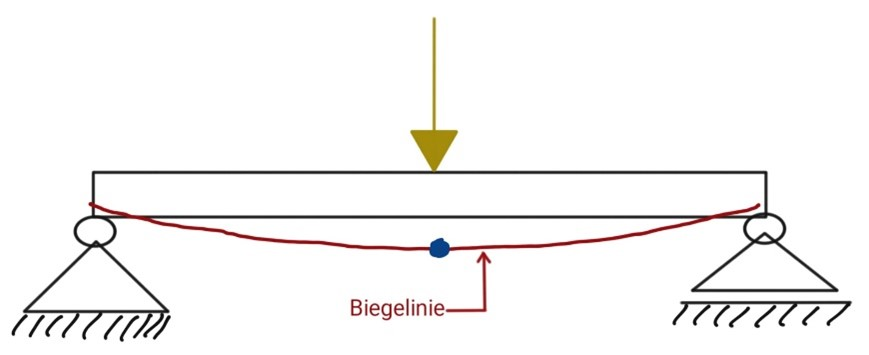
\includegraphics[width=0.8\textwidth]{papers/balken/images/teil1/Biegelinie1.jpg}
\end{center}
\label{Abbildung der Biegelinie aufgrund einer Einzellast}

\textbf{Biegemoment (M)}
Das Biegemoment, auch Schnittmoment genannt, ist eine Beanspruchung, bei dem ein Drehmoment erzeugt wird.
Diese Beanspruchung kann entweder durch eine vertikale Kraft mit einem Hebelarm ausgelöst werden
\begin{equation}
	M=
	F\cdot\ s
\end{equation}
\label{Formel für die Berechnung von Momenten}
oder durch ein bereits vorhandenes Drehmoment selbst.
. Biegemomente entstehen, wenn eine Kraft auf einen Körper einwirkt und eine Biegung oder Drehung auszulösen versucht.
\begin{center}
	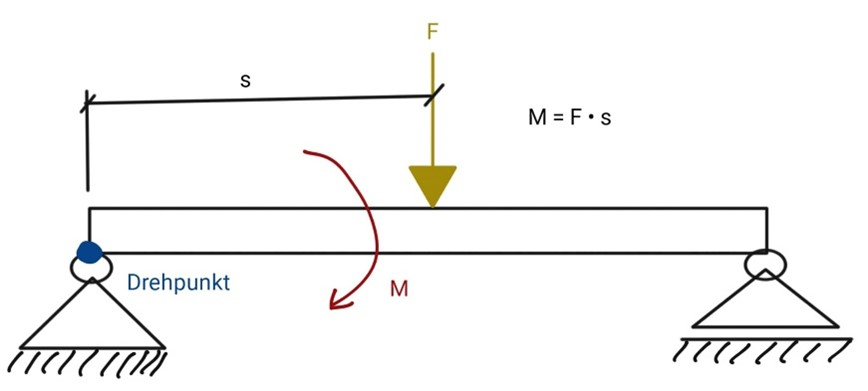
\includegraphics[width=0.8\textwidth]{papers/balken/images/teil1/Biegemoment.jpg}
\end{center}
\label{Die Abbildung zeigt einen Balken, der von einer einzigen Last belastet wird, was zu auftretenden Momenten führt.}

\textbf{Biegesteifigkeit (σB,R)}
Die Biegesteifigkeit besagt wie widerstandsfähig ein Material und Form gegen eine Biegebeanspruchung ist.
Sie beschreibt die Fähigkeit eines Balkens, sich unter äusserliche Einwirkung eines Biegemomentes zu verformen.
\begin{equation}
	\sigma_{B,R}=
	E\left(x\right)\cdot\ I\left(x\right)=
	\frac{M(x)}{W(x)}
\end{equation}
\label{Formel für die Biegesteifigkeit einer Bauteils}
E(x) = Elastizitätsmodul
I(x) = Flächenträgheitsmoment
M(x) = Moment 
W(x) = Widerstandsmoment

\textbf{E-Modul (E)}
Das E-Modul ist eine Materialkonstante, welches die Steifigkeit eines Materials beschreibt.
Er gibt an, wie viel Spannung ein Material aushalten kann, bis das Material eine bestimmte Dehnung erfährt.
Der E-Modul wird definiert als
\begin{equation}
	E=
	\frac{\sigma}{\varepsilon}
\end{equation}
σ = Spannung
ε = Dehnung

\textbf{Festlager}
Ein Festlager ist ein Lager, das fähig ist, Kräfte in horizontaler und vertikaler Rich-tung aufzunehmen, jedoch keine Momente aufnehmen kann.
Aufgrund dieser Eigenschaften werden Festlager als 2-wertige Auflager bezeich-net, da sie zwei Auflagerreaktionen haben (Querkräfte und Horizontalkräfte) und nur einen Freiheitsgrad (Momente) besitzen.
\begin{center}
	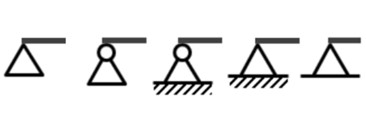
\includegraphics[width=0.8\textwidth]{papers/balken/images/teil1/Festlager.jpg}
\end{center}
\label{Die Abbildung zeigt verschiedene Darstellungsweisen eines Festlagers in der Baustatik.}

\textbf{Flächenträgheitsmoment (I)}
Das Flächenträgheitsmoment gibt die Trägheit eines Körpers an gegenüber einer Änderung seiner Drehbewegung.
Anders ausgedrückt gibt es an, wie widerstandsfähig ein Bauteil gegen Biegung ist.
Diese Trägheit wird ausschliesslich durch die Form des Körpers bestimmt, weshalb das Flächenträgheitsmoment von der Geometrie des Querschnittes abhängt.

\textbf{Lasten}
Lasten sind Kräfte oder Belastungen, die auf einen Körper bzw. statischen System wirken.
Sie können aufgrund von Gewichtskräfte, externe Kräfte, thermische Belastungen und vieles mehr auftreten.
Lasten gibt es in vier verschiedene Arten.
\begin{center}
	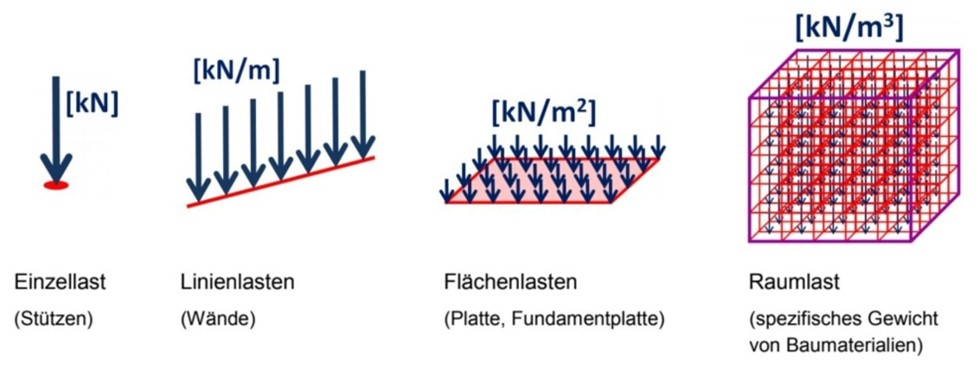
\includegraphics[width=0.8\textwidth]{papers/balken/images/teil1/Lasten.jpg}
\end{center}
\label{Die Abbildung zeigt verschiedene Lasttypen, die in der Baustatik vorkommen.}

\textbf{Loslager}
Loslagern besitzen die Fähigkeit Querkräfte aufzunehmen und werden deshalb als statisch 1-wertige Auflagern genannt.
Da sie Horizontalkräfte und Momenten nicht aufnehmen können, besitzen sie zwei Freiheitsgrade.
\begin{center}
	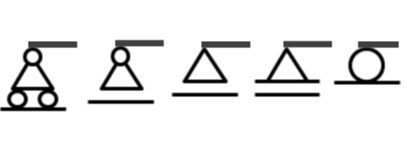
\includegraphics[width=0.8\textwidth]{papers/balken/images/teil1/Loslager.jpg}
\end{center}
\label{Festlagern werden typischerweise mit den folgenden Symbolen dargestellt.}

\textbf{Nulllinie}
Die Nulllinie ist eine Referenzlinie, von der Berechnungen durchgeführt werden. Sie dient als Bezugspunkt für Abständen und Winkeln.
Die Nulllinie ist dort wo die Fasern des Baumaterials neutral, sprich unbelastet sind.
Bei einachsigen Beanspruchungen liegt die Nulllinie typischerweise in der Mitte des Querschnitts.
Bei schräger Biegung verläuft die Nulllinie jedoch schräg durch den Querschnitt.

\textbf{Querkraft (Q)}
Querkräfte sind Kräfte, die senkrecht zur Längsrichtung eines Bauteils wirken.
Sie üben Druck- und Zugkräfte seitlich auf den Bauteil aus, was zu Biegungen führen kann.

\textbf{Widerstandsmoment (W)}
Das Widerstandsmoment kann mithilfe des Flächenträgheitsmoments berechnet werden.
Es gibt an, welchen Widerstand ein belastetes Bauteil den inneren Spannungen entgegensetzt.
\begin{equation}
	W=
	I/c
\end{equation}
\label{Formel für den Widerstandsmoment.}

W = Widerstandsmoment
I = Flächenträgheitsmoment
c = Abstand des äusseren Fasermittelpunkts zu der neutralen Faser

\subsection{Einführung in die Balkengleichung}
Wirken Lasten auf einen Balken, so führt es zu einer Verformung der Balken aufgrund von auftretenden Momenten um die y-Achse.
Die Balkentheorie analysiert diese Verformungen unter verschiedenen Lastszenarien und bestimmt dadurch die Biegelinie des Balkens, welche den Verlauf der Verformung entlang seiner Länge beschreibt.
Wir wollen nun die Balkengleichung der Biegelinie u(x) herleiten.

Wir betrachten einen schmalen Balke, welche seine Länge L entlang der x-Achse verläuft.
Allfällige Momente wirken um den y-Achse im Uhrzeigersinn und erzeugen eine positive Biegelinie u(x) mit der Öffnung gegen oben.
D.h. u(x) > 0.
Dabei verwenden wir die Euler-Bernoulli-Balkengleichung (EBB), die gültig ist, wenn reine Biegung so-wie Querkraftbiegung auftreten.
Für die EBB werden ausschliesslich Querschnitte betrachtet, die lotrecht zur Nulllinie liegen (im unbelasteten Zustand).